% !TeX root = main.tex
\section{Computational Methods and Agent Capability Assessment}
\subsection{Computational Settings and Scientific Tasks}
Calculations were performed using ORCA 6.1.1 and organized through OPI 2.0.0 and the unified execution interface.
The local resource allocation comprised four CPU cores, a memory limit of 1024 MiB for the computational process tree,
and an ORCA MaxCore setting of 192 MiB per process.
MaxCore is an internal ORCA memory parameter and was configured separately from the total memory limit on the process tree.

Table~\ref{tab:task-overview} lists the methods actually used for the seven test problems.
All systems for which calculations were completed were neutral singlets.
The r$^{2}$SCAN-3c calculations used the built-in def2-mTZVPP basis set~\cite{r2scan3c};
other methods and basis sets are reported individually according to the calculations performed,
with the basis sets following the def2 definitions~\cite{def2}.
Vertical excitations were calculated using full linear-response TDDFT~\cite{tddft},
and the aqueous environment was represented by the CPCM continuum model~\cite{cpcm}.
Except for the explicitly identified geometry optimizations and constrained optimizations,
all results correspond to specified fixed geometries.

\subsection{Design of the Agent Capability Assessment}
\label{sec:agent-evaluation-design}
The seven problems below assess \textbf{the ability of the Auto-ORCA agent to translate scientific requests
into actual calculations and interpretable results}.
The assessment covers the full process, from task interpretation, preservation of conditions,
and input preparation to the organization of results.
The molecules and properties were selected to impose distinct operational requirements:
some problems require a structure to be obtained before a property can be calculated;
others require management of a finite candidate set, preservation of comparable conditions,
organization of multiple excited states, or tensor analysis.
Together, these problems constitute a set of capability checks that examine both whether the agent can initiate and complete
actual ORCA calculations and whether its deliverables clearly identify the calculated system, conditions, and scope of the conclusions.

The test set includes operations relevant to potential energy surfaces as well as property calculations.
T1--T3 address local structure determination, comparison of candidate geometries,
and constrained calculations along an internal coordinate, respectively.
These are common components of potential energy surface exploration.
T4, T5, H1, and H2 extend the assessment to excited states, environmental changes, and response tensors,
testing whether the same execution interface can support different forms of output.
Task identifiers serve only to associate problems with their results;
capability assessments are based on the actual inputs, outputs, and geometry records.
Table~\ref{tab:agent-capability-design} specifies the capabilities targeted by each problem and the evidence that requires examination.

\begin{figure}[htbp]
  \centering
  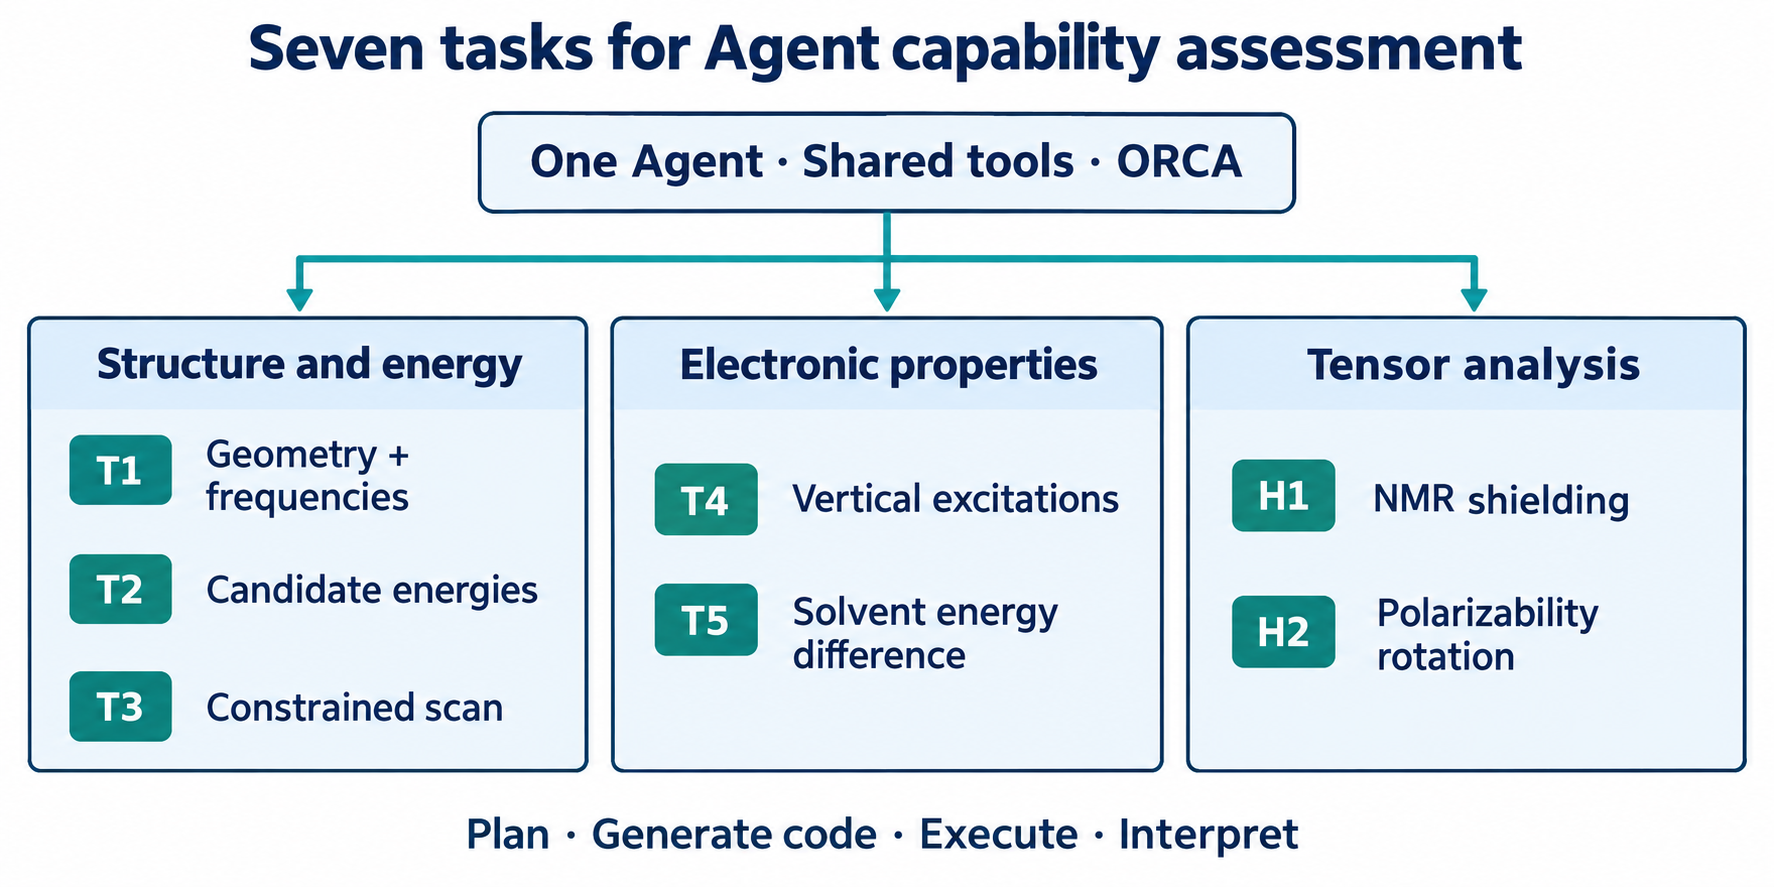
\includegraphics[width=\linewidth]{agent-capability-map.png}
  \caption{Scope of the agent capability assessment across seven problems.
  All problems use the same task organization and ORCA execution mechanism,
  while examining distinct operational requirements for structures and energies, electronic properties, and tensor analysis.
  The diagram illustrates the assessment design; the extent of completion is determined by the actual results.}
  \label{fig:agent-capability-map}
\end{figure}

\begin{table}[htbp]
  \centering\small
  \caption{Design of the agent capability assessment.
  The table lists the intended assessment dimensions; the extent of completion is reported with the individual results.}
  \label{tab:agent-capability-design}
  \begin{tabularx}{\linewidth}{lYY}
    \toprule
    Task & Principal capability & Evidence to examine\\
    \midrule
    T1 & Organize optimization--frequency dependencies and preserve structural provenance
       & Optimization convergence, final geometry, frequency count, and imaginary frequencies\\
    T2 & Organize a finite set of candidate calculations, associate identifiers, and standardize energy units
       & Candidate geometries, individual energies, reference candidate, and unit conversions\\
    T3 & Generate a loop for constrained calculations and maintain correspondence between target inputs and actual geometries
       & Constraint inputs, outputs at each point, final dihedral angles, and incomplete points\\
    T4 & Configure native property calculations and associate outputs across excited states
       & Method and TDA settings, convergence records, state-resolved energies, and oscillator strengths\\
    T5 & Preserve comparable geometries and methods when changing the environment
       & Geometries in both environments, basis and solvent settings, and the sign of the energy difference\\
    H1 & Parse atom-resolved tensors while preserving units and component ordering
       & Atom indices, complete shielding matrices, isotropic values, and units of ppm\\
    H2 & Organize calculations before and after rotation and check tensor consistency
       & Both molecular orientations, rotation definition, polarizability tensors, and comparison residuals\\
    \bottomrule
  \end{tabularx}
\end{table}

\FloatBarrier

Results can be examined at three levels.
First, the actual method, geometry, charge, and multiplicity are checked to associate each result with a well-defined computational problem.
Second, the raw ORCA output is examined for normal termination and the requested numerical values are checked for actual preservation.
Third, the interpretation is assessed against the available evidence.
For example, the lowest single-point energy in a finite candidate set must not be described as the global minimum conformer,
and an electronic energy difference at a fixed geometry must not be described as a free energy.
The first two levels establish the provenance of the computational system and its outputs;
the third determines the extent to which those outputs answer the scientific question.

Accordingly, Table~\ref{tab:agent-capability-design} specifies the dimensions covered by the assessment,
rather than a set of capabilities that have all been demonstrated successfully.
The completed calculations provide examples of diverse task formulations, execution, and numerical delivery.
A more complete assessment still requires individual verification of dependencies, geometric correspondence, and property interpretation.
The seven-problem success rate also lacks the statistical evidence provided by repeated trials or comparison systems
and therefore cannot estimate the probability of success on unseen tasks.
Future evaluations can repeat these problems under identical goals and conditions,
resolve the remaining verification gaps, and distinguish computational completion, verifiability of results,
and fulfillment of the scientific goals.

\subsection{Calculation Success Rate and Interpretation of Results}
Normal-termination records in the raw ORCA output serve as evidence that a calculation has completed.
Each problem in this study is classified as \textbf{successful} if a corresponding ORCA calculation has terminated normally
and its numerical results have been retained; a problem with no actual numerical result is classified as \textbf{incomplete}.
This classification includes the six completed points in T3 despite the uncomputed endpoint and the limitations of angle verification.
\begin{equation}
  R_{\mathrm{calc}}=\frac{N_{\mathrm{success}}}{N_{\mathrm{questions}}}
  =\frac{6}{7}\approx85.7\%.
  \label{eq:success-rate}
\end{equation}
The denominator is the set of seven problems, with each problem counted once.
Scientific conclusions are interpreted separately using the available evidence on convergence, geometry, method, and property.
Normal termination alone does not establish a global minimum conformer, a correct torsional barrier,
or a response property that can be compared directly with experiment.

Relative electronic energies are referenced to a specified member of the candidate set.
Energy conversions use $1\,\Eh=2625.4996394799$ kJ mol$^{-1}$.
Electronic energies, vibrational frequencies, excitation energies, and shielding tensors retain the precision
of the original output or verification record.
Raw data and provenance records support inspection and reuse~\cite{fair}.
This report presents existing computational results; the reported success rate is not interpreted as a success probability
for arbitrary new tasks, and energy differences without independent references are not used to assess methodological accuracy.

\subsection{Scope of the Evaluation}
The calculation success rate across the seven problems indicates whether the agent has produced actual computational results for those problems.
Assessing numerical accuracy additionally requires confirmation that each calculated value and its independent reference
refer to the same system, geometry, physical quantity, and theoretical conditions.
For tasks with reliable reference values, the coverage of valid matches and the error over the matched subset can be reported separately:
\begin{equation}
  \mathrm{Coverage}=\frac{N_{\mathrm{matched}}}{N_{\mathrm{target}}},
  \qquad
  \mathrm{MAE}_{\mathrm{matched}}=
  \frac{1}{N_{\mathrm{matched}}}\sum_{i\in\mathcal M}|y_i-y_i^{\mathrm{ref}}|.
  \label{eq:coverage-accuracy}
\end{equation}
Here, $\mathcal M$ includes only targets whose correspondence has been established,
and $y_i$ and $y_i^{\mathrm{ref}}$ are expressed in the same units.
If $N_{\mathrm{matched}}=0$, the error is not evaluable.
This formulation specifies the conditions required for future accuracy comparisons.
No independent high-accuracy references are available in this study; consequently, no empirical MAE is reported,
and energy differences between distinct methods or geometries are not treated as numerical errors.

\section{Results of the Agent Capability Assessment}
% !TeX root = main.tex
\subsection{Overview of the Seven Test Cases}
The following seven scientific questions were used to evaluate the task organization and execution capabilities of Auto-ORCA Agent;
their intended capability coverage is summarized in Table~\ref{tab:agent-capability-design}.
Table~\ref{tab:task-overview} summarizes the methods actually used and the results obtained for each case.
T1--T5 and H1 were classified as successful calculations, whereas H2 remained incomplete, yielding a calculation success rate of $6/7=85.7\%$.
The numerical results and their scientific interpretation are presented below.

\begin{table}[H]
  \centering\small
  \caption{Methods actually used and results obtained for the seven test cases.
  Success indicates that an ORCA calculation terminated normally and produced the corresponding numerical results.
  }
  \label{tab:task-overview}
  \begin{tabularx}{\linewidth}{l>{\raggedright\arraybackslash}p{2.6cm}>{\raggedright\arraybackslash}p{3.1cm}>{\raggedright\arraybackslash}p{1.8cm}Y}
    \toprule
    ID & Question & Actual method & Status & Principal results\\
    \midrule
    T1 & Ethanol optimization and frequencies & r$^{2}$SCAN-3c & Success & Converged optimization; 21 positive frequencies and no imaginary frequencies\\
    T2 & Candidate energies for \textit{n}-hexane & r$^{2}$SCAN-3c single-point calculations & Success & Energy ranking of six candidate geometries\\
    T3 & Dihedral scan of \textit{n}-butane & r$^{2}$SCAN-3c constrained optimization & Success & Six converged points; actual angles remain unverified\\
    T4 & Vertical excitations of acetone & PBE0/def2-SVP, LR-TDDFT & Success & Five singlet excitation energies and oscillator strengths\\
    T5 & Environmental energy differences for ethanol & B3LYP/def2-TZVP and def2-SVP & Success & Gas-phase--CPCM water electronic energy differences with two basis sets\\
    H1 & Nuclear magnetic shielding of HCN & PBE0/def2-TZVP, GIAO & Success & Full shielding tensors for the C, N, and H nuclei\\
    H2 & Formaldehyde polarizability and rotational consistency & No actual calculation results & Incomplete & No polarizability values obtained\\
    \bottomrule
  \end{tabularx}
\end{table}

\subsection{T1: Geometry Optimization and Vibrational Frequencies of Ethanol}
\paragraph{Question}
Optimize the geometry of ethanol and use its vibrational frequencies to assess whether the resulting structure is a local minimum.

\paragraph{Method}
Geometry optimization and vibrational frequency calculations were performed using r$^{2}$SCAN-3c with its built-in def2-mTZVPP basis set for a neutral singlet in the gas phase.

\paragraph{Results}
\textbf{Successful calculation.} The geometry optimization converged, giving an optimized electronic energy of $-155.002345492244\,\Eh$.
The calculation yielded 21 positive vibrational frequencies, six zero-frequency translational and rotational modes after projection, and no imaginary frequencies.
All positive frequencies are listed in Table~\ref{tab:t1-frequencies}.
These results support assignment of the structure as a local minimum at the employed level of theory; they do not establish that it is the global minimum-energy conformer.
The optimized coordinates are retained in the XYZ file associated with the corresponding ORCA output.

\begin{table}[H]
  \centering\small
  \caption{The 21 positive vibrational frequencies of ethanol, in cm$^{-1}$.}
  \label{tab:t1-frequencies}
  \begin{tabular}{rrrrrrr}
    \toprule
    270.90 & 298.95 & 425.86 & 811.51 & 882.13 & 1052.13 & 1066.45\\
    1134.41 & 1282.25 & 1371.13 & 1396.18 & 1418.25 & 1483.33 & 1487.57\\
    1509.53 & 2969.59 & 3004.65 & 3061.83 & 3088.36 & 3105.66 & 3819.31\\
    \bottomrule
  \end{tabular}
\end{table}

\subsection{T2: Single-Point Electronic Energies of Candidate \textit{n}-Hexane Conformers}
\paragraph{Question}
Compare the electronic energies of candidate \textit{n}-hexane geometries and determine their relative energy ordering within the calculated set.

\paragraph{Method}
Single-point calculations were performed separately for six stored candidate geometries using r$^{2}$SCAN-3c for neutral singlets in the gas phase.
Relative energies were referenced to cand\_05.

\paragraph{Results}
\textbf{Successful calculation.} Electronic energies were obtained for all six candidates, as reported in Table~\ref{tab:t2-energies}.
Within this set, cand\_05 had the lowest energy, whereas cand\_03 was higher by 12.608656~kJ~mol$^{-1}$.
These are single-point results for candidate geometries; they do not demonstrate that all six conformers underwent DFT optimization,
nor do they establish the global minimum-energy conformer or a free-energy ordering.

\begin{table}[H]
  \centering\small
  \caption{Single-point electronic energies of six candidate \textit{n}-hexane geometries.}
  \label{tab:t2-energies}
  \begin{tabular}{lrr}
    \toprule
    Candidate & Electronic energy / $\Eh$ & Relative energy / kJ mol$^{-1}$\\
    \midrule
    cand\_05 & $-236.992066202851$ & 0.000000\\
    cand\_04 & $-236.991445556657$ & 1.629506\\
    cand\_01 & $-236.991444090308$ & 1.633356\\
    cand\_00 & $-236.991421448668$ & 1.692802\\
    cand\_06 & $-236.991245997872$ & 2.153448\\
    cand\_03 & $-236.987263819406$ & 12.608656\\
    \bottomrule
  \end{tabular}
\end{table}

\subsection{T3: Dihedral Scan of \textit{n}-Butane}
\paragraph{Question}
Obtain the electronic energies of \textit{n}-butane at different target dihedral angles through constrained optimization and examine the variation in torsional potential energy.

\paragraph{Method}
The main calculations employed r$^{2}$SCAN-3c for a neutral singlet in the gas phase, with constrained optimization at specified target dihedral angles.
An additional B3LYP/def2-TZVP calculation point is reported separately, together with the result of its geometry verification.

\paragraph{Results}
\textbf{Successful calculation.} Normal ORCA termination and optimization convergence were recorded for all six r$^{2}$SCAN-3c calculation points;
the results are given in Table~\ref{tab:t3-energies}.
The first column contains only the target-angle labels specified in the inputs.
The actual angles reported by the generated script conflict with these input labels and have not yet been confirmed through independent geometry verification.
Consequently, the energies are genuine computational outputs, but the labels cannot be treated as verified actual dihedral angles or used to establish a torsional barrier.
In particular, the high energy associated with the $+120^\circ$ label cannot be directly interpreted as a reliable physical barrier.

\begin{table}[H]
  \centering\small
  \caption{Six constrained optimization points for \textit{n}-butane.
  Angles denote input target labels; relative energies are the stored numerical values.
  }
  \label{tab:t3-energies}
  \begin{tabular}{rrr}
    \toprule
    Input target angle / $^\circ$ & Electronic energy / $\Eh$ & Relative energy / kJ mol$^{-1}$\\
    \midrule
    $-180$ & $-158.392470368263$ & 0.000000\\
    $-120$ & $-158.387146187943$ & 13.978634\\
    $-60$ & $-158.391526560891$ & 2.477966\\
    $0$ & $-158.383528626170$ & 23.476541\\
    $+60$ & $-158.391526702130$ & 2.477595\\
    $+120$ & $-158.358972460497$ & 87.948745\\
    \bottomrule
  \end{tabular}
\end{table}

The input target angle for the B3LYP/def2-TZVP calculation point was $-180^\circ$.
Independent geometry verification gave an actual angle of $179.999995786^\circ$, consistent with the target under angular periodicity;
the converged electronic energy was $-158.397118300397\,\Eh$.
Because this point was obtained using a different method, it is excluded from the relative energies in Table~\ref{tab:t3-energies}.

\subsection{T4: The First Five Singlet Vertical Excitations of Acetone}
\paragraph{Question}
Obtain the excitation energies, wavelengths, and oscillator strengths of the first five singlet vertical excitations of acetone.

\paragraph{Method}
Five singlet excited states were calculated at a fixed, prepared geometry using PBE0/def2-SVP for a neutral singlet in the gas phase,
with full linear-response TDDFT (LR-TDDFT; \code{TDA=false}).
Oscillator strengths were taken from the length-gauge output of ORCA.

\paragraph{Results}
\textbf{Successful calculation.} Convergence was recorded for both the SCF and response calculations; numerical results for the five excited states are listed in Table~\ref{tab:t4-excitations}.
The lowest singlet vertical excitation energy was 4.197061~eV, corresponding to a wavelength of 295.4~nm.

\begin{table}[H]
  \centering\small
  \caption{The first five singlet vertical excitations of acetone.
  Oscillator strengths $f$ are dimensionless.
  }
  \label{tab:t4-excitations}
  \begin{tabular}{crrr}
    \toprule
    Excited state & Excitation energy / eV & Wavelength / nm & Oscillator strength $f$\\
    \midrule
    $S_{1}$ & 4.197061 & 295.4 & 0.000007493\\
    $S_{2}$ & 7.464499 & 166.1 & 0.023781213\\
    $S_{3}$ & 8.406988 & 147.5 & 0.001899769\\
    $S_{4}$ & 8.572306 & 144.6 & 0.060276158\\
    $S_{5}$ & 8.640904 & 143.5 & 0.004121254\\
    \bottomrule
  \end{tabular}
\end{table}

\subsection{T5: Electronic Energy Differences between Gas-Phase Ethanol and Ethanol in CPCM Water}
\paragraph{Question}
Compare the electronic energies of ethanol at the same geometry in the gas phase and in a CPCM water environment.

\paragraph{Method}
Calculations employed B3LYP for a neutral singlet with the def2-TZVP and def2-SVP basis sets, respectively.
For each basis set, the gas-phase and aqueous-environment calculations used the same initial geometry; this geometry was not the optimized structure from T1.
The energy difference was defined as $\Delta E=E_{\mathrm{water}}-E_{\mathrm{gas}}$.

\paragraph{Results}
\textbf{Successful calculation.} Two ORCA calculations, one in the gas phase and one in CPCM water, were completed for each basis set.
Table~\ref{tab:t5-energies} reports the electronic energies, and Table~\ref{tab:t5-differences} reports their differences.
The negative signs indicate that, for the corresponding model and fixed geometry, the electronic energy in the aqueous environment was lower than that in the gas phase.
These quantities are \textbf{electronic energy differences, not hydration free energies}.

\begin{table}[H]
  \centering\small
  \caption{Electronic energies of ethanol in the gas phase and in CPCM water.}
  \label{tab:t5-energies}
  \begin{tabular}{lrr}
    \toprule
    Basis set & Gas-phase electronic energy / $\Eh$ & CPCM water electronic energy / $\Eh$\\
    \midrule
    def2-TZVP & $-155.002778990957$ & $-155.009740144896$\\
    def2-SVP & $-154.817054999208$ & $-154.823380641772$\\
    \bottomrule
  \end{tabular}
\end{table}

\begin{table}[H]
  \centering\small
  \caption{Electronic energy differences for ethanol in water relative to the gas phase.}
  \label{tab:t5-differences}
  \begin{tabular}{lrr}
    \toprule
    Basis set & $\Delta E$ / $\Eh$ & $\Delta E$ / kJ mol$^{-1}$\\
    \midrule
    def2-TZVP & $-0.006961153939$ & $-18.276507$\\
    def2-SVP & $-0.006325642564$ & $-16.607972$\\
    \bottomrule
  \end{tabular}
\end{table}

\subsection{H1: GIAO Nuclear Magnetic Shielding Tensors of HCN}
\paragraph{Question}
Obtain the nuclear magnetic shielding tensor and isotropic shielding of each atom in HCN.

\paragraph{Method}
Calculations were performed at a fixed initial geometry using PBE0/def2-TZVP and the GIAO method for a neutral singlet in the gas phase.
The atom order was C$_0$, N$_1$, and H$_2$.

\paragraph{Results}
\textbf{Successful calculation.} The total electronic energy was $-93.345070922944\,\Eh$.
The isotropic shielding values printed by ORCA are listed in Table~\ref{tab:h1-isotropic}; the full total shielding tensors are given in Eq.~\eqref{eq:h1-tensors}.
The tensor components are expressed in ppm, with both rows and columns ordered as X, Y, and Z; the three decimal places of the original output are retained.

\begin{table}[H]
  \centering\small
  \caption{Isotropic nuclear magnetic shielding values for HCN.}
  \label{tab:h1-isotropic}
  \begin{tabular}{cr}
    \toprule
    Atom & Isotropic shielding / ppm\\
    \midrule
    C$_0$ & 79.051\\
    N$_1$ & $-34.068$\\
    H$_2$ & 29.850\\
    \bottomrule
  \end{tabular}
\end{table}

\begin{equation}
  \begin{aligned}
    \bm{\sigma}_{\mathrm{C}_0}&=\begin{pmatrix}
      279.306 & -0.724 & -0.000 \\
      -1.638 & -21.077 & 0.000 \\
      -0.000 & 0.000 & -21.076
    \end{pmatrix},\\[0.8em]
    \bm{\sigma}_{\mathrm{N}_1}&=\begin{pmatrix}
      340.398 & -1.842 & -0.000 \\
      -0.044 & -221.291 & 0.000 \\
      0.000 & 0.000 & -221.309
    \end{pmatrix},\\[0.8em]
    \bm{\sigma}_{\mathrm{H}_2}&=\begin{pmatrix}
      39.712 & 0.055 & -0.000 \\
      -0.114 & 24.919 & -0.000 \\
      -0.000 & -0.000 & 24.920
    \end{pmatrix}.
  \end{aligned}
  \label{eq:h1-tensors}
\end{equation}
Isotropic shielding is one-third of the tensor trace; the tabulated values were taken directly from the summary printed by ORCA and were not recalculated from the rounded matrices.
These quantities have not been converted using a reference compound and therefore cannot be directly described as experimental chemical shifts.
H$_2$ denotes the index of the hydrogen atom and is unrelated to the task identifier H2 in the following subsection.

\subsection{H2: Static Polarizability and Rotational Consistency of Formaldehyde}
\paragraph{Question}
Obtain the static polarizability tensors and isotropic polarizabilities of formaldehyde in two orientations, and assess their physical consistency under rotation.

\paragraph{Method}
The geometries and rotation procedure were prepared, with the intention of calculating the polarizability in each orientation and comparing the results after coordinate transformation.

\paragraph{Results}
\textbf{Incomplete.} No actual ORCA polarizability values have been obtained.
Consequently, neither the polarizability tensors and isotropic polarizabilities in the two orientations nor a rotational consistency comparison is available.
The prepared geometries and rotation procedure do not constitute calculation results.

\paragraph{Analysis of the Failure}
The execution records indicate that interruption occurred primarily during task orchestration and data handoff before the calculation.
In the recorded attempts, an identity-description file was incorrectly bound as an XYZ geometry input, causing the rotation preprocessing script to terminate abnormally during coordinate parsing.
The identification and use of diagnostic information did not yield an effective repair; the corresponding runs terminated upon reaching either the model-call limit or the finite allowance for plan revisions.


\subsection{Agent Token Usage and Costs for Runs Producing Computational Results}
\label{sec:token-cost}
To characterize the model resources required for autonomous task organization,
Table~\ref{tab:token-cost} lists six runs that produced the ORCA numerical results reported above.
Input, output, and total token counts were accumulated from the provider's per-call usage records
and cross-checked against the usage records for the corresponding runs.
The counts cover each entire agent run, including task interpretation, input preparation, planning decisions,
code repair, analysis, and reporting.
ORCA itself consumes computational resources rather than language-model tokens.
Because model calls and ORCA jobs do not correspond one-to-one, their counts are listed separately.

\begin{table}[H]
  \centering\small
  \setlength{\tabcolsep}{4pt}
  \caption{Agent token usage and estimated off-peak costs for runs that produced ORCA results.
  Token usage records are complete for all six runs.
  Costs are estimated uniformly using DeepSeek Flash rates and the recorded cache usage, and are expressed in USD.}
  \label{tab:token-cost}
  \begin{tabular*}{\linewidth}{@{\extracolsep{\fill}}lrrrrrr@{}}
    \toprule
    Task & \shortstack[r]{ORCA\\jobs} & \shortstack[r]{Model\\calls} & \shortstack[r]{Input\\tokens} & \shortstack[r]{Output\\tokens} & \shortstack[r]{Total\\tokens} & \shortstack[r]{Off-peak\\estimate}\\
    \midrule
    T1 & 1 & 21 & 311,695 & 86,697 & 398,392 & 0.079900\\
    T2 & 6 & 12 & 181,958 & 49,010 & 230,968 & 0.049813\\
    T3 & 6 & 14 & 231,346 & 107,149 & 338,495 & 0.092519\\
    T4 & 1 & 23 & 367,183 & 75,633 & 442,816 & 0.087719\\
    T5 & 2 & 12 & 192,013 & 62,392 & 254,405 & 0.063885\\
    H1 & 1 & 24 & 368,095 & 117,100 & 485,195 & 0.114298\\
    \bottomrule
  \end{tabular*}
\end{table}

All six cost estimates use the rates for \code{deepseek-flash}.
The rates for cached input, uncached input, and output are 0.003, 0.15, and 0.60 USD per million tokens, respectively.
Let $N_{\mathrm{hit}}$ denote the cached input tokens already included in the total input count.
The cost is then estimated as
\begin{equation}
  C_{\mathrm{off\text{-}peak}}=
  \frac{p_{\mathrm{hit}}N_{\mathrm{hit}}
  +p_{\mathrm{miss}}(N_{\mathrm{input}}-N_{\mathrm{hit}})
  +p_{\mathrm{out}}N_{\mathrm{output}}}{10^6}
  \quad\text{USD}.
  \label{eq:token-cost}
\end{equation}
Here, $p_{\mathrm{hit}}$, $p_{\mathrm{miss}}$, and $p_{\mathrm{out}}$ are the three Flash off-peak rates.
Cache-hit counts are obtained from the provider's usage records and are not added again to the input or total token counts.

\section{Discussion}
\subsection{Execution Across Tasks and Scientific Interpretation}
The six successful problems cover geometry optimization, harmonic frequencies, single-point energies,
constrained optimization, vertical excitations, environmental energy comparisons, and nuclear magnetic shielding.
These results demonstrate that generated programs can organize different types of calculations through a common ORCA interface.
The numerical results for the \textit{n}-hexane candidates and acetone excitations, reported in the preceding tables,
illustrate the organization of calculations over a candidate set and the processing of multiple excited states, respectively.

The results directly relevant to potential energy surfaces have different evidential scopes.
The converged optimization and absence of imaginary frequencies in T1 support a local minimum.
T2 provides a ranking of single-point energies for a finite set of candidate geometries.
T3 retains six converged constrained-optimization points but lacks independently verified correspondence between target and actual angles.
The available results therefore support the execution of operations relevant to potential energy surfaces,
but do not establish a completed global potential energy surface search or a reliable, complete torsional barrier profile.

Property calculations likewise require precise identification of the physical quantities involved.
T4 describes vertical excitations at a fixed prepared geometry; T5 provides electronic energy differences at fixed geometry;
and H1 provides absolute nuclear magnetic shielding values.
H2 has not produced tensor values, so rotational consistency cannot yet be tested.
Subsequent validation should first address these specific gaps, followed by repeated calculations under identical conditions
and comparisons with independent references to assess reproducibility and accuracy.

\subsection{Preserving Goals and Connecting Evidence for Continued Exploration}
A further contribution of Auto-ORCA is to maintain continuity between the user's scientific question and the final deliverable.
Natural-language requests typically combine goals, conditions, and expected interpretations,
whereas a single ORCA calculation can provide only part of the required information.
When each result enters the next decision cycle, it must therefore be assessed against the current question:
which structure produced it, under which conditions, what has been answered, and what further evidence is required.
This stepwise connection decomposes extended tasks into executable and checkable operations while preserving the overall research objective.

Auto-ORCA maintains the correspondence among scientific goals, computational conditions, and results,
and selects subsequent calculations, analyses, or repairs using new evidence.
The seven tests demonstrate the feasibility of organizing diverse molecular calculations through this process.
Its efficiency and reliability still require assessment through controlled comparisons and repeated trials under identical conditions.

In the final report, structured results and natural-language explanations serve complementary purposes.
Tables and matrices preserve numerical values, units, and object identifiers,
while the accompanying text explains computational methods, physical meaning, and applicability.
This combination allows readers to understand the principal findings and trace the results back to the raw artifacts for inspection.

\subsection{Limitations and Future Evaluation}
The present dataset is limited in size, and the problems differ in both computational steps and physical quantities.
Counting each problem once cannot directly measure the quality of individual model decisions,
the completion rate of all required steps, or numerical accuracy.
The study does not include comparison systems evaluated under common conditions,
distributions from repeated trials, or independent high-accuracy references.
It therefore does not support performance rankings of models or architectures.

Further evaluation can proceed in three directions.
First, repeated execution with identical inputs and resources can test the stability of results and stopping behavior.
Second, unseen tasks can assess whether generated code generalizes to new combinations of operations.
Third, independent references or deterministic checks for the physical quantities can distinguish execution errors
from errors arising from the electronic-structure approximation itself.
For scan tasks, final geometries and endpoints should be checked first;
environmental comparisons should retain common conditions;
and tensor tasks should verify components, units, and coordinate transformations together.

Comparisons of the underlying mechanisms also require controlled conditions.
The separation of goals from plans, retention of repair information, and organization of feedback can be studied as independent factors.
Each comparison must preserve the original scientific problem and minimum requirements.
Only then can improvements in task organization be distinguished from changes in inputs, budgets, or acceptance criteria.

\Needspace{9\baselineskip}
\section{Conclusions}
This study presents Auto-ORCA, which combines generic tools and generated code within a single-agent decision loop
to perform DFT tasks through a unified ORCA interface.
The system separately preserves the original goals, actual computational conditions, and numerical evidence.
Among seven test problems, T1--T5 and H1 produced completed ORCA calculations and numerical results,
yielding a calculation success rate of $6/7=85.7\%$ under the definition adopted here.
H2 has not yet produced actual polarizability values.

At the workflow level, Auto-ORCA connects natural-language input, intent recognition, condition clarification,
knowledge retrieval, dependency planning, task code, managed execution, and result interpretation in a continuous process.
Successful results inform further progress toward the goals, failure diagnostics support targeted repairs,
and the final report links conclusions to the methods actually used and the raw artifacts.
This organization supports multistep calculations centered on a scientific question
and provides an explicit basis for further analysis and reuse of existing results.

The principal results include a converged ethanol structure with 21 positive vibrational frequencies,
single-point energies for six \textit{n}-hexane candidates, six constrained-optimization points for \textit{n}-butane,
five singlet excitations of acetone, gas-to-aqueous electronic energy differences with two basis sets,
and complete shielding tensors for the three nuclei in HCN.
The interpretation of each structure or property remains conditional on its supporting evidence:
a local minimum does not establish a global minimum, the angle correspondence in the \textit{n}-butane scan still requires verification,
and an environmental electronic energy difference is not a hydration free energy.
Future work should address geometric verification, sampling completeness, response-tensor validation,
and repeated trials to further assess the reliability of autonomous potential energy surface exploration.
